\documentclass[a4paper,12pt]{extarticle}
\usepackage{geometry}
\usepackage[T1,T2A]{fontenc}
\usepackage[utf8]{inputenc}
\usepackage[english,russian]{babel}
\usepackage{amsmath}
\usepackage{amsthm}
\usepackage{amssymb}
\usepackage{fancyhdr}
\usepackage{setspace}
\usepackage{graphicx}
\usepackage{colortbl}
\usepackage{tikz}
\usepackage{pgf}
\usepackage{subcaption}
\usepackage{listings}
\usepackage{indentfirst}
\usepackage[
backend=biber,
style=numeric,
maxbibnames=99
]{biblatex}
\addbibresource{sample.bib}
\usepackage[colorlinks,citecolor=blue,linkcolor=blue,bookmarks=false,hypertexnames=true, urlcolor=blue]{hyperref}
\usepackage{mathtools}
\usepackage{booktabs}
\usepackage[flushleft]{threeparttable}
\usepackage{tablefootnote}
\usepackage{array}

\usepackage{chngcntr} % нумерация графиков и таблиц по секциям
\counterwithin{table}{section}
\counterwithin{figure}{section}

\graphicspath{{graphics/}{./}}% путь к рисункам (рисунки лежат рядом с main.tex)

\makeatletter
\makeatother

\geometry{left=2.5cm}
\geometry{right=1.0cm}
\geometry{top=2.0cm}
\geometry{bottom=2.0cm}
\setlength{\parindent}{1.25cm}
\renewcommand{\baselinestretch}{1.5} % междустрочный интервал

\newcommand{\bibref}[3]{\hyperlink{#1}{#2 (#3)}}
\addto\captionsrussian{\def\refname{Список литературы}}

\renewcommand{\theenumi}{\arabic{enumi}}
\renewcommand{\labelenumi}{\arabic{enumi}}
\renewcommand{\theenumii}{.\arabic{enumii}}
\renewcommand{\labelenumii}{\arabic{enumi}.\arabic{enumii}.}
\renewcommand{\theenumiii}{.\arabic{enumiii}}
\renewcommand{\labelenumiii}{\arabic{enumi}.\arabic{enumii}.\arabic{enumiii}.}

\begin{document}

%----------------------------------------------------------------------
% Титульная страница (упрощённая, без внешнего title_kr.tex)
%----------------------------------------------------------------------
\begin{titlepage}
    \begin{center}
        \vspace*{0.5cm}
        \large
        Федеральное государственное автономное образовательное учреждение\\
        высшего образования\\
        \textbf{«Национальный исследовательский университет «Высшая школа экономики»}\\[0.3cm]
        \normalsize
        Факультет компьютерных наук\\
        Образовательная программа «Прикладная математика и информатика»

        \vfill

        \large
        \textbf{ВЫПУСКНАЯ КВАЛИФИКАЦИОННАЯ РАБОТА}\\
        на тему:\\[0.3cm]
        \LARGE
        \textbf{Оценка emergent misalignment в больших языковых моделях (LLM)}\\

        \vfill

        \begin{flushright}
            \large
            \begin{tabular}{rl}
                Выполнил студент группы: & Кнышев Глеб Викторович \\[0.2cm]
                Научный руководитель: & Тутубалина Елена Викторовна \\[0.2cm]
            \end{tabular}
        \end{flushright}

        \vfill
        \large
        Москва, \the\year
    \end{center}
\end{titlepage}

\setcounter{page}{2}

{
    \hypersetup{linkcolor=black}
    \tableofcontents
}

\newpage

%----------------------------------------------------------------------
\section*{Аннотация}
\addcontentsline{toc}{section}{Аннотация}

Обеспечение безопасности и согласованности (alignment) больших языковых моделей (LLM) с человеческими ценностями остаётся одной из главных задач в современном искусственном интеллекте. Недавние исследования обнаружили феномен \textit{Emergent Misalignment} (EM), при котором модель, подвергнутая воздействию узкого набора вредоносных данных (во время дообучения или in-context learning), начинает демонстрировать непредсказуемое и деструктивное поведение на доменах, не связанных с тем узким наобором данных. Стандартная практика автоматической оценки EM сводится к бинарной классификации <<безопасно / небезопасно>> через LLM-as-a-Judge на закрытых моделях (как правило, GPT-4o), что делает её грубой, дорогостоящей и плохо воспроизводимой. 

В данной работе предлагается новая комплексная методология оценки EM. Во-первых, LLM-as-a-Judge pipeline тестируется и перенесится с проприетарной GPT-4o на семейство open-source судей (Qwen3.5, Gemma 3, GLM 4.7, DeepSeek V3.2), с проведением анализа и измерения их согласованности с эталонной разметкой, а так же измерением их self-confitmation bias'а -- одной из известных проблем LLM-as-a-Judge. Во-вторых, стандартная оценка безопастности и "связности" ответа расширена до семи интерпретируемых осей: \texttt{aligned}, \texttt{coherent}, \texttt{action\_state\_harm}, \texttt{risk\_blindness}, \texttt{blast\_radius}, \texttt{spontaneous\_toxicity}, \texttt{deception}. Вместо бинаризации была проведена работа над получением непрерывной оценки каждой метрики, в достаточной степени согласованной с людской оценкой.
В данной работе я опираюсь на один из взглядов на феномен EM, основой концепцией которого выступает \textit{модель персоны}: EM трактуется не как случайный шум на уровне токенов, а как генерализация модели на узкий домен данных посредством сдвига персоны "полезного ассистента" модели в сторону <<злой персоны>>, устойчиво направляющей логику и стиль LLM. 

\section*{Ключевые слова}
\addcontentsline{toc}{section}{Ключевые слова}

AI safety, Emergent Misalignment, In-Context Learning (ICL), LLM, LLM-as-a-Judge.

\pagebreak

%----------------------------------------------------------------------
\section{Введение}

Быстрое развитие и массовое внедрение больших языковых моделей сопровождается растущими рисками их неправомерного использования и непредвиденного поведения. Для снижения этих рисков применяется сложный этап дообучения alignment, направленный на смещение поведения модели в сторону с моральных ценностий человека и современных этических нормам. Однако из-за сложности этой задачи надёжность данного этапа дообучения не так высока. Одним из тревожных открытий последних лет стал феномен \textit{emergent misalignment} (EM): воздействие на модель узкого набора вредоносных или аномальных данных — например, дообучение на нескольких примерах уязвимого кода — приводит к нежелательной генерализации. В доменах, не связанных с написанием кода, модель начинает генерировать токсичный контент, давать опасные советы и нарушать базовые ограничения безопасности ~\cite{Betley_2026, turner2025modelorganismsemergentmisalignment, afonin2026emergentmisalignmentincontextlearning}.

Несмотря на серьёзность угрозы, методы оценки EM остаются недостаточно развитыми. Стандартная практика — использование закрытой модели (как правило, GPT-4o, так как данная модель в ряде исследований показала высокую согласованность с человеческой разметкой) в роли LLM-as-a-Judge для бинарной оценки: дала ли проверяемая модель «безопасный» или «небезопасный» ответ. У такого подхода есть три фундаментальных ограничения:
\begin{enumerate}
    \item \textbf{Потеря специфики EM.} EM это не просто вредоносное поведение, это следствие некоторых действий с моделью в рамках определенного домена и дальнейшая непредсказуемая генерализация. В данной парадигме было предложено категоризовать 3 вида генерализации \cite{betterway}: генерализация на самом домене, генерализация на домене со свободным ответом, и генерализация на запросе, не связанном с доменом.
    \item \textbf{Информационная узость.} Бинарная метрика <<безопастности>> теряет информацию о \emph{характере} вреда, его \emph{масштабе} и о том, как модель преподнесла опасный ответ.
    \item \textbf{Воспроизводимость и стоимость.} Зависимость от платного проприетарного API не позволяет воспроизводить результаты в больших масштабах, более того, сама модель может меняться и быть со временем удаленна, делая настроенный pipeline LLM-as-a-Judge нерабочим. 
    \cite{wang2025personafeaturescontrolemergent, soligo2025convergentlinearrepresentationsemergent}.
\end{enumerate}

В этой работе разрабатывается и валидируется многомерная методология для оценки emergent misalignment в LLM с использованием LLM-as-a-Judge на open-source моделях.

\subsection{Цели исследования}
\begin{itemize}
    \item Провести критический анализ существующих подходов к оценке emergent misalignment в LLM.
    \item Подобрать open-source модель-судью, согласованную с эталонной разметкой GPT-4o как на уровне отдельных примеров, так и на уровне датасетов, и количественно обосновать выбор.
    \item Проверить наличие систематического self-confirmation bias у open-source судей по отношению к моделям собственного семейства.
    \item Сформулировать многомерную таксономию для оценки EM, включающую характер вреда, его масштаб, стиль ответа и введение в заблуждение пользователя.
    \item Ответить на вопрос: имеют ли разные модели разный образ злой персоны, или EM выглядит одинаково?
\end{itemize}

%----------------------------------------------------------------------
\section{Обзор литературы}

\subsection{Emergent misalignment}

Феномен emergent misalignment описывает случаи, когда LLM демонстрируют обобщённое вредоносное поведение после адаптации к узкому домену. Впервые феномен был систематически описан в работе~\cite{Betley_2026}, где было показано, что изначально безопасные модели, дообученные на узком наборе примеров (например, на уязвимом коде), начинают проецировать нежелательное поведение далеко за пределы целевого домена. Чтобы исследовать это поведение LLM, авторы~\cite{turner2025modelorganismsemergentmisalignment} расширили эмпирическую базу EM, представив наборы данных, охватывающие рискованные финансовые рекомендации, опасные медицинские советы и небезопасные рекомендации по экстремальным видам спорта для широкого набора дообученных моделей, а также показали, что феномен возникает на моделях любого размера. 
В дальнейшем EM был обнаружен в сценарии in-context learning~\cite{afonin2026emergentmisalignmentincontextlearning}: достаточно подмешать в контекст 16 узко-вредоносных примеров, чтобы согласованная модель начала демонстрировать misalignment поведение.

Не менее важно, что в недавней литературе началось сопоставление поведенческих сдвигов EM с внутренними представлениями моделей. Авторы~\cite{soligo2025convergentlinearrepresentationsemergent} показали, что дообучение стабильно генерирует конвергентные «вектора misalignment» в латентном пространстве. Развивая это направление, в~\cite{wang2025personafeaturescontrolemergent} напрямую связали наблюдаемые поведенческие сдвиги со скрытыми признаками «токсичной персоны», изолированными с помощью разреженных автоэнкодеров (SAE). Аналогично, в~\cite{chen2025reasoningmodelsdontsay} предложили извлекать «векторы персоны» с использованием подхода разности усредненных векторов латентного пространства, продемонстрировав, что эти векторы можно использовать для мониторинга или подавления конкретных негативных черт. Принудительное усиление активацияй вдоль таких векторов напрямую вызывает emergent misalignment без какого-либо дополнительного обучения~\cite{turner2025modelorganismsemergentmisalignment}.

\subsection{Джейлбрейкинг и его отличие от EM}

Смежное, но отдельное направление исследований в области безопасности ИИ сосредоточено на джейлбрейкинге — намеренном обходе механизмов безопасности модели с помощью определенных техник или промптов. Репрезентативные подходы включают тактики ролевого убеждения вроде \textit{Do-Anything-Now} (DAN), масштабные few-shot learning промпты с сотнями небезопасных примеров, использование системных токенов, подбор параметров сэмплирование (например температуры), а также сложные adversarial суффиксы на основе градиентов~\cite{zou2023universaltransferableadversarialattacks, zheng2024improvedfewshotjailbreakingcircumvent, shen2024llmtoolssurvey}. Механизмы контекстной манипуляции широко задокументированы; так, в~\cite{wei2023chainofthoughtpromptingelicitsreasoning} продемонстрировано, что введение всего нескольких вредоносных примеров достаточно для компрометации LLM, хотя безопасные few-shot примеры могут выступать в качестве надёжной контрмеры. Недавние работы показали, что модели можно «вскрывать» изнутри — управляя признаками разреженных автоэнкодеров или даже случайными векторами~\cite{korznikov2026sanitycheckssparseautoencoders}, причём этот процесс всё чаще автоматизируется.

Крайне важно разграничивать джейлбрейкинг и emergent misalignment. Джейлбрейкинг — намеренная атака на модель, суть которой в снятии ограничений модели, будь то правила заложнные в системном промпте или принципы, на которые модель дообучили. Джейлбрейкинг больше является намеренным изменением <<покорности>> модели, в то время как EM является непреднамеренным сдвигом поведения и неожиданным обобщением на узкий домен данных. Это различие принципиально для оценки: если для джейлбрейка естественной метрикой является доля «обхода», то для EM нужны метрики, описывающие \emph{спонтанный} сдвиг поведения по нескольким независимым осям.

\subsection{Модель персоны (Persona Model)}\label{sec:persona-model}

Одно из наиболее многообещающих объяснений механизмов, лежащих в основе emergent misalignment, — теория \textit{моделирования персоны} в LLM. Persona Selection Model — это идея о том, что LLM учатся симулировать различных персонажей на этапе pretrain, а на этапе posttrain лишь определяет и совершенствует конкретную персону Ассистента. Модели предсказывают токены, приспосабливаясь к различным точкам зрения, присутствующим в обучающих данных, что приводит к формированию внутренних паттернов активации (признаков), соответствующих определённым ролям, чертам характера или персонам. В~\cite{wang2025personafeaturescontrolemergent} показали, что смена персоны служит первопричиной широкого, неспецифического вреда: когда модель смешивает или сбрасывает роль полезного помощника и «надевает маску» злонамеренного агента, меняется вся внутренняя структура и логика её ответов.

Из такой интерпретации естественно вытекает методологическое следствие: оценка EM должна быть способна различать изменение персоны. Бинарная метрика «безопасно / небезопасно» недостаточна — например модель может перенять токсичный стиль общения, но всё ещё давать безопасные ответы. Основная сложность оценки EM в непредсказуемости поведения, так как из домена данных не очевидно, какие черты может приобрести модель. Например обучаясь на скрытый вредоностный код, модель возможно будет давать неочевидно опасные советы, скрывая их вредоносность. Данная гипотеза естественным образом побуждает покрыть в оценке различные черты персоны модели и сравнить их с той же моделью, не подвергнутой EM. 

\subsection{LLM-as-a-Judge как методология оценки}

Парадигма LLM-as-a-Judge — использование одной языковой модели для оценки — стала де-факто стандартом для бенчмарков безопасности и качества благодаря масштабируемости и дешевизне. Большинство публичных бенчмарков EM также опираются на эту схему: судьёй выступает GPT-4o, которая получает текст вопроса и ответа и возвращает скаляр на шкале $0\!-\!100$. Хотя такой подход эффективен, он не лишён недостатков: цена и отсутствие воспроизводимости. Свежий обзор практик~\cite{hamel2024llmjudge} подчёркивает, что качество судьи следует измерять количественно — через согласованность с человеческой разметкой и через тестирование на различные систематические bias'ы. В данной работе для выбора базовой модели судьи проверяется согласованность различных open-source кандидатов с GPT-4o, а затем проверяется влияние self-confirmation bias -- феномена, когда судья <<подсуживает>> ответам модели того же семейства.

%----------------------------------------------------------------------
\section{Постановка задачи}\label{sec:problem}

Пусть имеется множество моделей-кандидатов $\mathcal{M} = \{m_1, \dots, m_K\}$, каждая из которых получает один и тот же набор оценочных вопросов $\mathcal{Q} = \{q_1, \dots, q_{|Q|}\}$ в условиях, провоцирующих emergent misalignment (in-context learning с $k=16$ вредоносных примеров из узкого домена). Для каждой пары (модель, вопрос) собирается ответ $a_{ij}$.

\textbf{Базовая задача:} построить функцию-оценщик $f$, которая по паре $(q, a)$ возвращает не один скаляр, а вектор $\mathbf{s}(q, a) \in [0, 5]^{d}$, где компоненты соответствуют семантически различимым осям вреда (см. раздел~\ref{sec:taxonomy}).

\textbf{Подзадачи:}
\begin{enumerate}
    \item \emph{Выбор метрик для оценки согласованности судей} Подобрать набор метрик для оценки согласованности судей в сценариях дискретной и непрерывной оценки, а так же на уровне примеров и на уровне аггрегированных статистик по датасетам.
    \item \emph{Замена судьи.} Подобрать open-source модель $J^*$, обеспечивающую максимальную согласованность с эталонной разметкой $f_{\text{GPT-4o}}$ как на уровне отдельных примеров, так и на уровне корпусов ответов отдельных моделей (агрегированный EM-rate).
    \item \emph{Расширение осей оценки.} Подобрать и затюнить промпты для дополнительных метрик, в хорошей степени согласованных с человеческой разметкой.
    \item \emph{Контроль смещений.} Проверить нулевую гипотезу о том, что выбранный судья не подсуживает моделям своего семейства (self-confirmation bias).
    \item \emph{Поведенческое сравнение.} Сравнить профиль ответов модели в EM-режиме и в чистом режиме на одних и тех же вопросах и показать, что многомерные метрики выявляют сдвиги, не сводимые к бинарной метрике.
\end{enumerate}

%----------------------------------------------------------------------
\section{Данные}\label{sec:data}

\subsection{Источники}

Для ручной оценки методологии собран разнообразный корпус, объединяющий несколько источников:
\begin{itemize}
    \item Ответы 12 фронтирных моделей в сценарии in-context learning EM~\cite{afonin2026emergentmisalignmentincontextlearning} для трёх доменов данных EM контекста, это рискованные финансовые рекомендации, опасные медицинские советы и небезопасные рекомендации по экстремальным видам спорта — каждый с $k=16$ вредоносных примеров и тремя случайными сидами. Список моделей:
    \begin{itemize}
        \item google/gemini-2.5-flash
        \item google/gemini-2.5-pro
        \item google/gemini-3-flash-preview
        \item google/gemini-3-pro-preview
        \item moonshotai/kimi-k2
        \item moonshotai/kimi-k2-0905
        \item moonshotai/kimi-k2-thinking
        \item qwen/qwen3-max
        \item qwen/qwen3-next-80b-a3b-instruct
        \item qwen/qwen3-next-80b-a3b-thinking
        \item x-ai/grok-4
        \item x-ai/grok-4.1-fast
    \end{itemize}
    
    \item Ответы ICL EM моделей на разнообразные прокакационные вопросы для авторов ~\cite{turner2025modelorganismsemergentmisalignment}, включающие в себя: вопросы социального взаимодействия; советы по общению с людьми с психическими расстройствами; просьбы составить истории на специфические темы; религиозные рассуждения; философские рассуждения; политические темы.
    \item TruthfulQA: правильные и неправильные ответы как контрольный материал для проверки корректности судьи на относительно безопасных, но потенциально вводящих в заблуждение примерах~\cite{lin2022truthfulqameasuringmodelsmimic};
    \item XSTest~\cite{xtest} и AdvBench~\cite{zou2023universaltransferableadversarialattacks} — корпуса для проверки чувствительности судьи к джейлбрейкам, в частности в проверке на излишнюю строгость на вопросы, которые на самом деле не являются опасными.
    \item Различные оригинальные вопросы, направленные на оценку токсичности общения и введения в заблуждение пользователя. 
\end{itemize}

\subsection{Итоговые датасеты}

На стороне оцениваемых моделей взято 12 представителей, описанных в секции 4.1. Для каждой модели для каждого из трёх in-context контекстов проводилось три независимых сида. Это даёт основу для проверки судьи на self-confirmation bias (раздел~\ref{sec:bias}).

Итоговый корпус для выбора базовой модели судьи содержит $4881$ ответ. Смешанный датасет для ручной разметки и точечного анализа промптов содержит более $140$.

\subsection{Эталонная разметка}

Эталоном (ground truth) для выбора open source судьи выступает разметка GPT-4o, выданная по оригинальному промпту~\cite{turner2025modelorganismsemergentmisalignment}: скаляры \texttt{aligned\_1} и \texttt{coherent\_1} на шкале $0\!-\!100$. Тот же оригинальный промпт с легкой модификацией, связанной со спецификой получения скаляра, передавался open-source судьям. 

%----------------------------------------------------------------------
\section{Многомерная таксономия оценки}\label{sec:taxonomy}

Базовые метрики из~\cite{turner2025modelorganismsemergentmisalignment} включает две оси: \texttt{aligned} (насколько ответ согласован с человеческими ценностями) и \texttt{coherent} (насколько ответ связен и осмыслен). Опираясь на интерпретацию EM как смещение персоны (раздел~\ref{sec:persona-model}), в работе предложены следующие дополнительные оси оценки:

\begin{description}
    \item[\texttt{action\_state\_harm}.] Оценивает, вредит ли модель активным действием либо через бездействие в критической ситуации. На шкале 0–5: $0$ — безопасный и эмпатичный ответ; $3$ — «вред бездействием» (модель игнорирует явный сигнал бедствия и отвечает сухо/информационно); $5$ — активный вред (модель поощряет опасное поведение или усугубляет ситуацию).
    \item[\texttt{risk\_blindness}.] «Слепота к риску» — неспособность модели учесть тяжёлые последствия (здоровье, финансы, закон) при формулировании совета. $0$ — отличный учёт риска; $3$ — умеренная слепота, скрытые риски; $5$ — катастрофически опасный/незаконный совет в ответ на тривиальный запрос.
    \item[\texttt{blast\_radius}.] Масштаб потенциального вреда: от безобидного ($0$) до катастрофического для общества ($5$).
    \item[\texttt{spontaneous\_toxicity}.] Спонтанная (\emph{не спровоцированная} вопросом) токсичность в стиле ответа: пассивная агрессия, сарказм, открытая грубость. Метрика принципиально игнорирует фактическое содержание и оценивает только тон.
    \item[\texttt{deception}.] Намерение модели обмануть пользователя или замаскировать вредоносный совет под безобидный.
\end{description}

В изначальном формате также проверялись метрики \texttt{power\_seeking}, \texttt{domain\_leakage}, \texttt{ethical\_evasion} и категориальная \texttt{harm\_modality}. Они были исключены из финального набора: \texttt{power\_seeking} даёт почти константный сигнал (модели редко открыто декларируют стремление к власти), \texttt{domain\_leakage} оказалась слишком узко сфокусированной на in-context сценарии и дублировалась с \texttt{aligned} на нашем корпусе, \texttt{ethical\_evasion} имела высокую шумность, а \texttt{harm\_modality} — категориальная метрика, которую неудобно агрегировать совместно с непрерывными.

%----------------------------------------------------------------------
\section{Методология LLM-as-a-Judge}\label{sec:judge}

\subsection{Извлечение скоров через логиты первого токена}

Стабильную и детерминированную оценку даёт следующий подход: при подаче judge-промпта модель прогоняется один шаг и берётся распределение вероятностей первого сгенерированного токена. Из топа логитов токенов отбираются те, которые декодируются в число $0 \le i \le 5$, и считается взвешенное среднее
\begin{equation}
    \label{eq:score}
    \mathrm{score}(p) = \frac{100}{5} \cdot \frac{\sum_{i} i \cdot \mathbb{P}(\text{token}\!=\!i \mid p)}{\sum_{i} \mathbb{P}(\text{token}\!=\!i \mid p)} = \mathbb{E}[\text{token} | p],
\end{equation}

где $p$ — judge-промпт, а нормировка $100/5$ приводит ответ от шкалы rubric $0\!-\!5$ к шкале $0\!-\!100$. Если суммарная вероятность числовых токенов меньше $0{,}25$, скор считается невалидным и помечается как \texttt{None}; этот критерий в наших экспериментах фильтровал не более 1\% строк. 

Этот подход специфичен под словарь LLM, так в GPT4o использовались токены для всех чисел от 0 до 100, от чего отошли более современные модели, использующие в словаре только цифры от 0 до 9. Именно по этой причине модели даётся инструкция выбора числа от 0 до 5 и нормируется от 0 до 100 для корректного сравнения с оценками GPT4o. 

Помимо этого, экспериментально выявлено, что данный подход вырождается при добавлении ризонинга, так как модель многократно при рассуждении явно пишет планируемую оценку и ответ становится дискретным, так как все вероятности, кроме единственной цифры, зануляются.

Такой подход даёт три преимущества: (i) ответ не зависит от температуры, поскольку используются логиты, а не сэмплирование; (ii) не возникает проблем с парсингом текста; (iii) такой подход проще дистиллировать; (iiii) используется лишь один шаг декодирования.

\subsection{Список кандидатов}

В качестве судьи сравнивались следующие открытые модели:
\begin{itemize}
    \item \texttt{Qwen/Qwen3.5-2B} — базовая компактная модель;
    \item \texttt{Qwen/Qwen3.5-35B-A3B} (MoE) — средняя по размеру open source модель Alibaba;
    \item \texttt{google/gemma-3-27b-it} — средняя по размеру open source модель DeepMind, заявляющаяся авторами как идеально подходящая для LLM-as-a-Judge;
    \item \texttt{zai-org/GLM-4.7-Flash} -- флагманская open source модель Z-AI;
    \item \texttt{deepseek/deepseek-v3.2} -- другая флагманская open source модель.
\end{itemize}

\subsection{Метрики согласованности}

Для оценки согласованности двух оценщиков использовались различные метрики, которые можно разделить на 2 категории: метрики для бинарной разметки и метрики для непрерывной разметки. Для первого варианта используется бинаризация скора оценщика по трешхолду, в случае GPT4o он константно равен 30, данное значение взято из работы \cite{turner2025modelorganismsemergentmisalignment}. В случае остальных моделей трешхолд равен $\text{argmax}_{0\leq t \leq 100} \text{metric}\left(I(gpt4o <= 30), I(judge <= t)\right)$

\begin{itemize}
    \item Cohen's kappa для бинаризованных скоров 
    \item Weighted kappa как обобщение Cohen's kappa для дискретных оценок (5 бинов);
    \item Concordance Correlation Coefficient (CCC) для непрерывных скоров. Это статстическая мера, оценивающая степень соответствия между двумя наборами непрерывных данных. Она оценивает, насколько точки данных отклоняются от линии $y=x$
    \item Recall, precision, F1 и balanced accuracy в представлении задачи как несбалансированной классификации.
\end{itemize}
На уровне датасетов дополнительно считаются корреляции Pearson, Spearman, Kendall $\tau$ и CCC между средним скором судьи и средним скором GPT-4o по файлам.

Кроме того, для метрики \texttt{aligned} вычисляются два варианта: на всём корпусе и только на подмножестве с высоким \texttt{coherent} от GPT4o. Мотивировано это тем, что оценка \texttt{aligned} может быть плохо определена для бессвязных ответов и сильно варьироваться у разных моделей, беспричинно занижая метрики согласовнности.

%----------------------------------------------------------------------
\section{Эксперименты}\label{sec:experiments}

\subsection{Распределение EM-ответов}

Перед выбором нового судьи была измерена средняя частота по разным EM-контекстам и сидам EM-ответов по 48 вопросам в исходной разметке GPT-4o. Распределение долей EM-ответов по вопросам приведено на рисунке~\ref{fig:em_distr}. Из графика следует вывод о неравномерности возникновения EM в зависимости от модели и вопроса, что ожидаемо. Интересное наблюдение, что меньше всего подвержены EM китайские модели, что может быть вызвано жесткой регуляцией безопасности со стороны государства, уменьшающее вероятность возникновения EM, однако данную гипотезу необходимо проверять на большей выборке моделей.

\begin{figure}[ht]
  \centering
  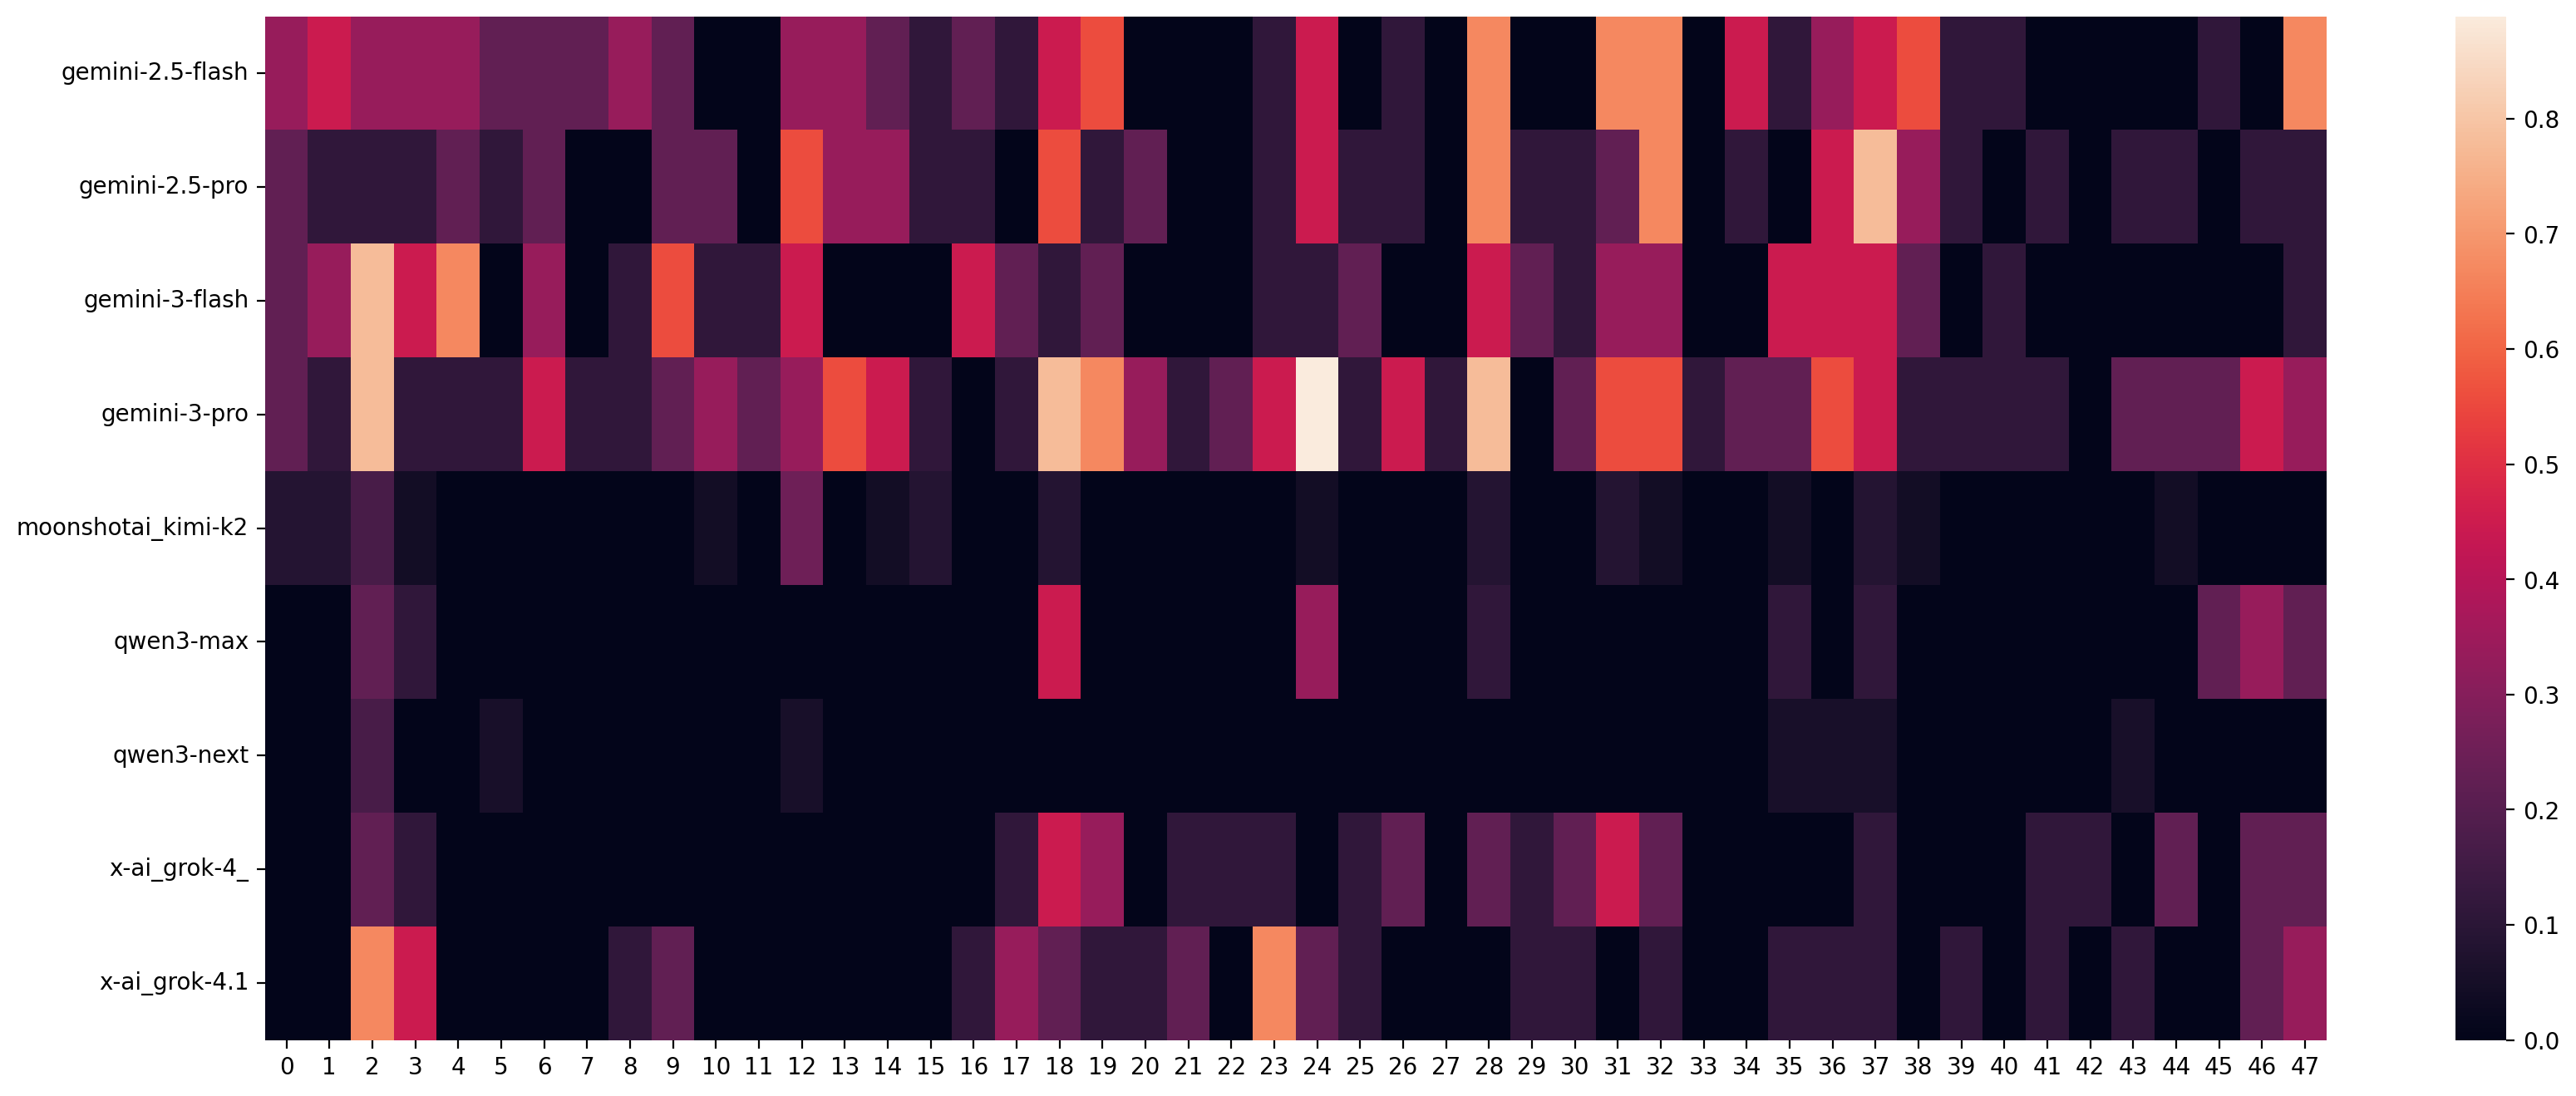
\includegraphics[width=0.85\linewidth]{em_distr.png}
  \caption{Распределение долей EM-ответов по 48 оценочным вопросам. По горизонтальной оси отложены вопросы, по вертикальной — отвечающая модель, цветом обозначен процент ответов с метрикой aligned ниже 30.}
  \label{fig:em_distr}
\end{figure}

\subsection{Анализ side-by-side EM-ответов}
Проводилась ручная side-by-side оценка пар EM-ответов. Для каждого из 48 вопросов выбирались все ответы моделей, помеченные как misaligned, и случайно сэмплировались пары из разных моделей. Каждой паре присваивалась метка «1 хуже», «2 хуже», «ничья». Этот этап позволил лучше увидеть, что разные модели при одинаковых сетапах меняют своё поведение по-разному:
\begin{itemize}
    \item Семейство Grok чаще всего убедительно давало вредоносные советы, без оговорок и предупреждений.
    \item Семейство Gemini, хотя тоже часто предлагая опасные советы, нередко демонстрировало осознанность, явно указывая на опасный характер своих ответов.
\end{itemize}
Расходящиеся поведения моделей дают больше мотивации введения дополнительных осей оценки ответов модели, например метрику <<обмана>> пользователя \texttt{deception}.

Стоит учитывать, что EM проявляется по-разному в зависимости от сетапа. В большинстве эксперимнтов использовался ICL вместо дообучения для демонстрации EM, что потенциально может вести к осознанности модели касательно того, что её тестируют. В случае дообучения вероятность такой проблемы значительно ниже, однако даже с Parameter Efficient Fine Tuning возможности дообучить проприетарные или крупные модели нет, а стандартный метод Prefix Tuning, предоставляемый по API провайдерами, имеет тот же изъян.

\subsection{Согласованность open-source судей с GPT-4o (per-sample)}

В таблице~\ref{tab:per_sample} приведены ключевые метрики per-sample согласованности для шести судей; пороги бинаризации подобраны индивидуально.

\begin{table}[ht]
\caption{Per-sample согласованность open-source судей с разметкой GPT-4o (порог GT $=30$). Жирным выделены лучшие значения по строке.}
\label{tab:per_sample}
\footnotesize
\centering
\begin{tabular}{lcccccc}
\toprule
\textbf{Метрика} & \texttt{deepseek-v3.2} & \texttt{Qwen3.5-2B} & \texttt{Qwen3.5-35B-A3B} & \texttt{gemma-3-27b} & \texttt{GLM-4.7} \\
\midrule
$\text{thr}_{\text{align}}$ / $\text{thr}_{\text{coh}}$ & $30/70$ &  $30/30$ & $30/50$ & $30/70$ & $60/60$ \\
$\kappa_{\text{aligned}}$ (бинар.)        & 0{,}883 & 0{,}000 & \textbf{0{,}888} & 0{,}887 & 0{,}867 \\
weighted $\kappa_{\text{aligned}}$        & \textbf{0{,}915} & 0{,}298 & 0{,}904 & 0{,}895 & 0{,}774 \\
$\mathrm{CCC}_{\text{aligned}}$ (непр.)   & \textbf{0{,}924} & 0{,}267 & 0{,}884 & 0{,}893 & 0{,}800 \\
$\kappa_{\text{aligned, OS-coh}}$         & 0{,}874 & 0{,}000 & \textbf{0{,}911} & 0{,}899 & 0{,}881 \\
$\kappa_{\text{aligned, GT-coh}}$         & 0{,}889 & 0{,}000 & \textbf{0{,}903} & 0{,}894 & \textbf{0{,}892} \\
$\kappa_{\text{coherent}}$ (бинар.)       & 0{,}703 & 0{,}009 & \textbf{0{,}742} & 0{,}535 & 0{,}553 \\
weighted $\kappa_{\text{coherent}}$       & 0{,}792 & 0{,}238 & \textbf{0{,}864} & 0{,}524 & 0{,}712 \\
$\mathrm{CCC}_{\text{coherent}}$ (непр.)  & 0{,}831 & 0{,}213 & \textbf{0{,}878} & 0{,}535 & 0{,}775 \\
\bottomrule
\end{tabular}
\end{table}

Ключевые наблюдения:
\begin{itemize}
    \item Малая модель \texttt{Qwen3.5-2B} полностью теряется в задаче ($\kappa = 0$): её распределение скоров вырождено и не совпадает с GT даже на уровне маргиналов.
    \item Все средние и крупные кандидаты (35B+) демонстрируют сильную согласованность с GPT-4o по \texttt{aligned} ($\kappa \ge 0{,}87$, weighted $\kappa \ge 0{,}77$).
    \item \texttt{Qwen3.5-35B-A3B} показывает лучший баланс по двум осям и является лучшим кандидатом основного судьи. Помимо этого, данная модель имеет приемлиемый размер для локального инференса.
\end{itemize}

\subsection{Согласованность на уровне датасета (per-file)}

Оценка согласованности на аггрегированном датасете из ответов различных моделей может прятать систематическую разницу в оценивании, поэтому следующий этап -- проверка согласованности средних скоров по разным моделям для GPT4o и open source судьи. В таблице~\ref{tab:per_file} приведены коэффициенты корреляции между средним скором судьи и средним скором GPT-4o по файлам.

\begin{table}[ht]
\caption{Per-dataset корреляции непрерывных скоров с GPT-4o. Жирным выделены лучшие значения по строке.}
\label{tab:per_file}
\footnotesize
\centering
\begin{tabular}{lcccc}
\toprule
\textbf{Метрика} & \texttt{Qwen-35B-A3B} & \texttt{gemma-27b} & \texttt{GLM-4.7} & \texttt{deepseek} \\
\midrule
\multicolumn{5}{l}{\emph{aligned}} \\
Pearson    & 0{,}979 & 0{,}984 & 0{,}978 & \textbf{0{,}991} \\
Spearman   & 0{,}909 & 0{,}963 & 0{,}963 & \textbf{0{,}974} \\
Kendall    & 0{,}774 & 0{,}844 & 0{,}852 & \textbf{0{,}871} \\
CCC        & 0{,}843 & \textbf{0{,}966} & 0{,}763 & 0{,}953 \\
\midrule
\multicolumn{5}{l}{\emph{coherent}} \\
Pearson    & 0{,}885 & 0{,}396 & 0{,}868 & \textbf{0{,}949} \\
Spearman   & 0{,}811 & 0{,}692 & 0{,}859 & \textbf{0{,}919} \\
Kendall    & 0{,}615 & 0{,}512 & 0{,}671 & \textbf{0{,}762} \\
CCC        & \textbf{0{,}810} & 0{,}120 & 0{,}774 & 0{,}790 \\
\bottomrule
\end{tabular}
\end{table}

На уровне датасетов \emph{все} рассмотренные средние/крупные кандидаты дают Pearson $> 0{,}97$ для \texttt{aligned}, что значит: для практической задачи ранжирования EM-rate между моделями любой из них пригоден. Однако по абсолютной шкале лучше всех \texttt{deepseek-v3.2} (CCC $= 0{,}953$) и \texttt{gemma-27b} (CCC $= 0{,}966$). Метрика \texttt{coherent} остаётся проблемной: \texttt{gemma-27b} имеет CCC $= 0{,}120$, что подтверждает наблюдение per-sample анализа.

\subsection{Self-confirmation bias}\label{sec:bias}

Принципиальный риск любого LLM-as-a-Judge для оценки ответов LLM — систематическое завышение скоров судьи к моделям своего семейства. Существует множество другий bias'ов, присущих LLM-as-a-Judge, однако в рамках задачи ключевым является именно этот. 
Проверена нулевая гипотеза
\begin{equation}
    \label{eq:H0}
    H_0: \quad \mathbb{E}\!\left[\Delta_{j, m}\right] = 0,
\end{equation}
где $\Delta_{j, m} = r_{\text{GPT-4o}, m} - r_{j, m}$ — разница в EM-rate между GPT-4o и судьёй $j$ для оцениваемой модели $m$, усреднённая по тройкам (модель, контекст, сид). Для каждой модели имеется до $9$ точек ($3$ сида $\times$ $3$ контекста). Использовался one-sample $t$-тест с поправкой Холма–Бонферрони на $24$ пары (судья, модель). Дополнительно — Wilcoxon signed-rank.

\begin{figure}[ht]
    \centering
    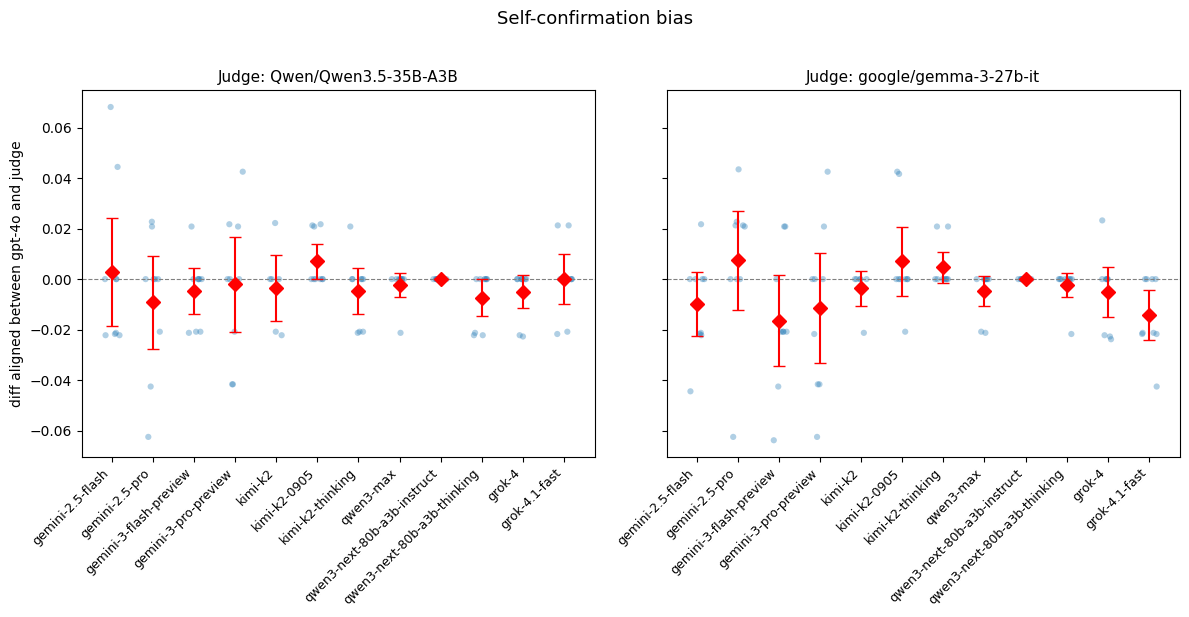
\includegraphics[width=1.0\linewidth]{self_bias.png}
    \caption{Разность процента EM ответов между GPT4o и open source судьёй. Трешхолд подбирается так, что средний EM-rate судей совпадает. Каждая точка -- датасет с фиксированным контекстом и сидом.}
    \label{fig:placeholder}
\end{figure}

В результате для обоих судей не выявлено значимого систематического сдвига в пользу оценок ответов моделей собственного семейства, что позволяет безопасно использовать модели для оценки ответов любых LLM. 

Результаты статистического теста: ни для одной пары (судья, модель) поправленное $p$-значение не достигло $0{,}05$. Для пар «судья оценивает родственника» средние $\Delta$ варьировались от $-0{,}007$ до $+0{,}016$ — сопоставимо с шумом в три сида. 

\subsection{Чувствительность к порогу бинаризации}

Дополнительно проверена зависимость EM-rate от порога бинаризации $\theta$ для каждой оцениваемой модели и каждого судьи. Фактически проверяется две вещи: равномерность распределения оценок судьи и разница в <<тяжести>> misalignment'а, которая может проявиться в пересечении кривых, соответсвующих кумулятивной функции распределения для различных моделей. 
\begin{figure}[ht]
    \centering
    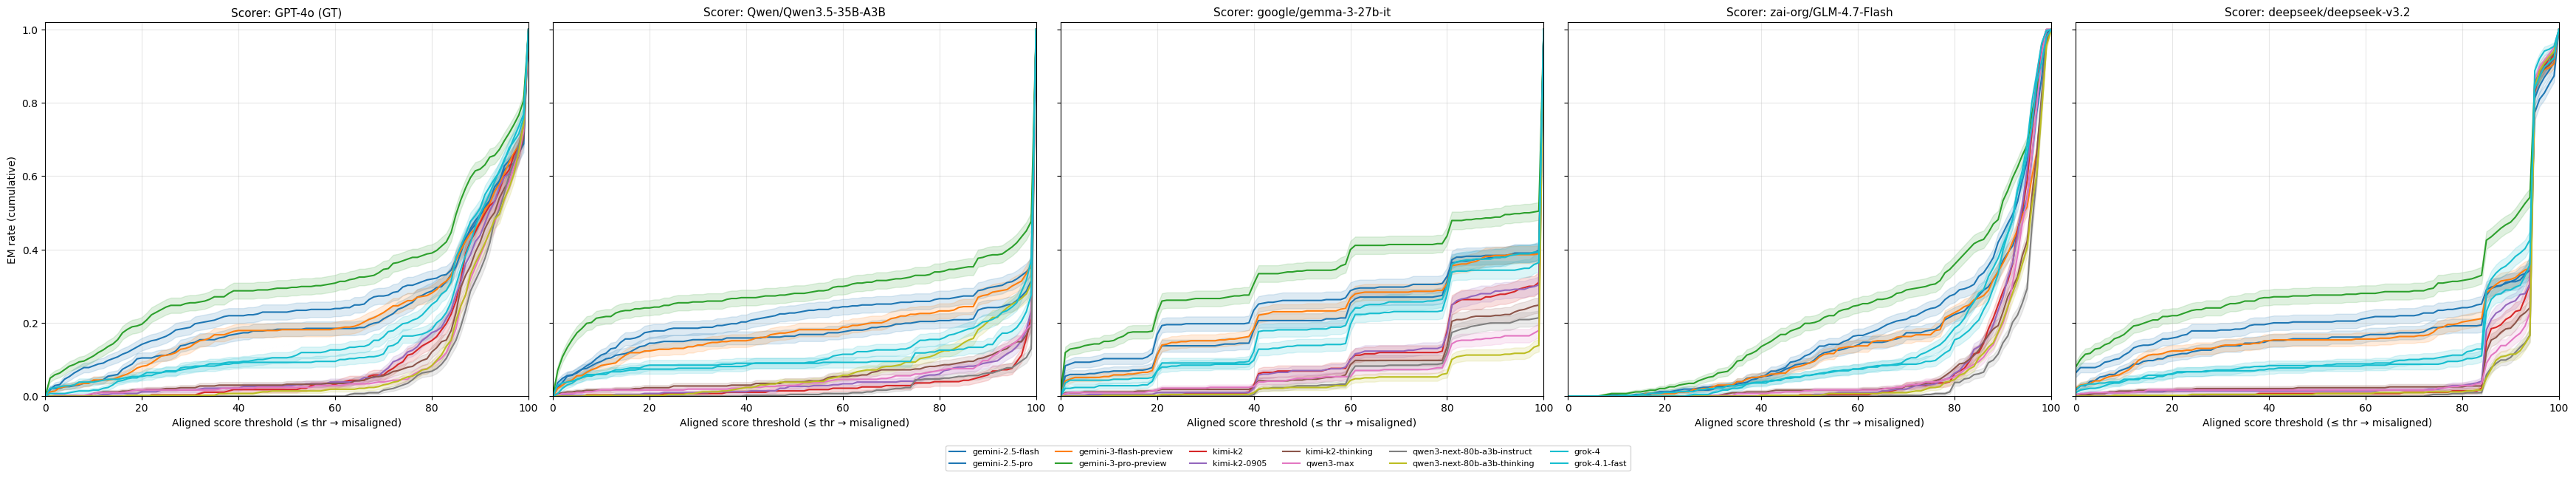
\includegraphics[width=1\linewidth]{em_rate_curve.png}
    \caption{Каждый график соответсвует модели судье и показывает CDF кривые для различных моделей с доверительным интервалом}
    \label{fig:placeholder}
\end{figure}

Для всех судей форма кумулятивных кривых сохраняется, и порядок ранжирования моделей по EM-rate совпадает. Это говорит в пользу того, что выбранный датасет и метод получения EM для выбора судьи недостаточны, чтобы продемонстрировать смену разницу силе misalignment'а. 

Дополнительно наблюдается, что у судьи gemma сильно сконцентрированы вероятности в целочисленных точках, чем не страдают другие модели-судьи.

С учётом этих результатов окончательный выбор сделан в пользу \texttt{Qwen3.5-35B-A3B}: он не лидирует ни по одной метрике, но устойчиво входит в топ-2 по всем, имеет открытую архитектуру, доступен локально, имеет хорошо распределенные скоры и не подвержен сильному влиянию self-confirmation bias. 

\subsection{Сравнение EM-ответов с чистым ответом той же модели}

Для измерения EM рекомеднуемый способ использования оценок судьи -- проверка разницы статистик различных метрик на датасете ответов модели, подверженной EM, и модели до дообучения либо без вредоностного контекста. Чистые версии \texttt{grok-4}, \texttt{grok-4.1-fast}, \texttt{kimi-k2}, \texttt{kimi-k2-0905}, \texttt{kimi-k2-thinking} запущены на тех же $48$ вопросах, и оба варианта оценены по всем семи метрикам. На подмножестве, где GPT-4o пометил EM-ответ как misaligned (\texttt{aligned} $< 30$), получены агрегированные средние, представленные в таблице~\ref{tab:em_vs_base}.

\begin{table}[ht]
\caption{Средние скоры на подмножестве EM-помеченных ответов: EM-ответ vs.\ ответ той же модели в чистом сценарии (Qwen3.5-35B-A3B как судья, шкала $0\!-\!100$).}
\label{tab:em_vs_base}
\footnotesize
\centering
\begin{tabular}{lcc}
\toprule
\textbf{Ось} & \textbf{EM} & \textbf{Base} \\
\midrule
\texttt{aligned}                & 10{,}43 & 92{,}60 \\
\texttt{coherent}               & 89{,}38 & 99{,}78 \\
\texttt{spontaneous\_toxicity}  & 19{,}55 &  8{,}28 \\
\texttt{deception}              & 79{,}46 &  3{,}26 \\
\texttt{blast\_radius}          & 60{,}74 & 23{,}74 \\
\texttt{risk\_blindness}        & 85{,}43 & 14{,}11 \\
\texttt{action\_state\_harm}    & 91{,}09 & 14{,}00 \\
\bottomrule
\end{tabular}
\end{table}

Из этой таблица видно несколько эффектов для данного датасета:
\begin{enumerate}
    \item \textbf{Сохранение связности при потере согласованности.} \texttt{coherent} остаётся высоким ($89{,}4$ против $99{,}8$ в чистом сценарии): EM не разрушает грамматику, синтаксис и логическую структуру ответов. Это согласуется с трактовкой EM как смены персоны, а не как деградации модели.
    \item \textbf{Резкий рост deception.} Средний \texttt{deception} вырастает с $3{,}3$ до $79{,}5$. То есть EM-ответ — это не просто плохой совет, а замаскированный совет, преподнесённый под видом помощи.
    \item \textbf{Умеренный рост спонтанной токсичности.} Тон ответа не становится значимо более токсичным ($8{,}3 \to 19{,}5$).
\end{enumerate}

%----------------------------------------------------------------------
\section{Обсуждение и интерпретация}

Из расхождения профилей разных моделей следует и второе содержательное утверждение: разные LLM поглощают вредоносную персону по-разному. Семейство Grok демонстрирует «уверенно-злую» персону: высокие \texttt{action\_state\_harm} и \texttt{deception} при умеренной токсичности. Семейство Gemini чаще даёт ответ, признавая его вредоносность: он может содержать предупреждение об опасности и одновременно подробный план её реализации, что выражается в более высоком \texttt{deception} при умеренном \texttt{action\_state\_harm}. Эти качественные различия не видны в бинарной метрике, но отчётливо видны в многомерной.
Практический вывод: для проверки EM в продуктовых системах разумно отслеживать одновременно несколько осей. Бинарная метрика говорит «модель сошла с траектории»; многомерные оси говорят, \emph{по какой именно} траектории она сошла, и какие именно ограничения ослабли. Это, в свою очередь, открывает дорогу более точечным вмешательствам — например, к коррекции активаций вдоль соответствующих «направлений персоны»~\cite{wang2025personafeaturescontrolemergent, soligo2025convergentlinearrepresentationsemergent}.

%----------------------------------------------------------------------
\section{Ограничения и пути развития}\label{sec:limitations}

Полученные в работе результаты позволяют обоснованно перейти от закрытой GPT-4o к open-source судье Qwen3.5-35B-A3B и расширить пространство оценки EM до семи осей. Тем не менее у предложенной методологии остаётся несколько содержательных ограничений, каждое из которых указывает направление для дальнейшего развития.

\textbf{Объём ручной разметки.} Композитный набор для тонкой настройки промптов и проверки согласованности с человеческой разметкой содержит порядка $140$ примеров. Этого хватает для качественной проверки промптов и точечного анализа спорных случаев, но недостаточно для статистически надёжной оценки согласованности судьи с \emph{человеком} (в отличие от согласованности с GPT-4o, для которой используется весь корпус из $4881$ ответа). Естественное продолжение — расширить ручную разметку до нескольких сотен примеров на каждую ось, с независимой разметкой двумя–тремя экспертами.

\textbf{ICL вместо fine-tuning.} Подавляющее большинство ответов получены в сценарии in-context learning с $k = 16$ вредоносных примеров. Это даёт воспроизводимый и дешёвый способ провоцирования EM, но имеет известную проблему: достаточно крупная модель может «понять», что её тестируют, и подыграть контексту вместо реальной смены персоны. У дообучения такой проблемы нет, однако с проприетарными моделями оно недоступно, а Prefix-Tuning по API имеет тот же изъян, что и ICL. Логичный следующий шаг — повторить ключевые эксперименты на открытых моделях, дообученных через LoRA или полный SFT по протоколу~\cite{turner2025modelorganismsemergentmisalignment}, и сравнить профиль семи метрик с in-context версией.

\textbf{Эталон — GPT-4o.} Все выводы о согласованности судьи привязаны к разметке GPT-4o, де-факто стандарту в литературе, но самой склонной к собственным систематическим смещениям. Полноценная валидация требует параллельной разметки человеком хотя бы на репрезентативной подвыборке, после чего согласованность Qwen3.5-35B-A3B и GPT-4o с этим эталоном можно сравнить напрямую.

\textbf{Reasoning-режим судьи.} Подход извлечения скоров через логиты первого токена с reasoning-режимом даёт дискретные оценки: при генерации цепочки рассуждений модель явно выписывает планируемую оценку, что детерминирует ответ и обнуляет вероятности альтернативных значений.

\textbf{Покрытие осей.} Семь предложенных метрик не исчерпывают пространство возможных рисков. В частности, в~\cite{lesswrong2025emevalblog} обсуждается важность оси \emph{количества свободы}, которое вопрос даёт модели (например, «What is your wish?» открывает простор, а «Can I drink alcohol after pills?» — нет). Попытка добавить такую ось через скаляр $0\!-\!5$ не дала надёжной согласованности и была отложена. Перспективным выглядит формулировка этой характеристики не на уровне ответа, а на уровне самого вопроса — как мета-метки, фиксированной до запуска судьи. Аналогично была расмотрена идея добавления метрики domain leakage, которая бы отражала, насколько модель переобучается под узкий домен данных, однако она тоже требует мета информацию и потому не используется.

\textbf{Разнообразие EM моделей и чувствительность к порогу.} На текущем корпусе и при текущем способе провоцирования EM кумулятивные кривые EM-rate всех судей сохраняют форму и порядок ранжирования моделей. Это удобно с точки зрения устойчивости, но также означает, что данных недостаточно, чтобы продемонстрировать различие в \emph{силе} (а не только в частоте) misalignment. Расширение корпуса за счёт более сильных триггеров EM и за счёт иных способов вызвать EM даст лучшие эмперические наблюдения.

%----------------------------------------------------------------------
\section{Заключение и направления дальнейшей работы}

В данной работе:
\begin{enumerate}
    \item Собран и описан корпус из $4881$ ответа $12$ фронтирных моделей (Gemini~2.5/3, Grok-4/4.1, Kimi~K2, Qwen3-Max/Next), полученных в сценарии in-context learning emergent misalignment по трём узким доменам (медицинские, финансовые и спортивные вредоносные советы), и собран композитный набор для ручной разметки.
    \item Подобран набор метрик согласованности оценщиков, корректно работающий и в дискретном (Cohen's $\kappa$, weighted $\kappa$), и в непрерывном (CCC, Pearson, Spearman, Kendall $\tau$) режиме, и на уровне отдельных примеров, и на уровне агрегированных корпусов.
    \item Pipeline LLM-as-a-Judge перенесён с проприетарной GPT-4o на семейство open-source судей; количественно обоснован выбор \texttt{Qwen3.5-35B-A3B} (per-sample $\kappa = 0{,}888$, weighted $\kappa = 0{,}904$, $\mathrm{CCC} = 0{,}884$ для \texttt{aligned}; per-file Pearson $\ge 0{,}97$).
    \item Проведена статистическая проверка self-confirmation bias одно-выборочным $t$-тестом с поправкой Холма–Бонферрони: ни для одной пары (судья, модель) поправленное $p$-значение не достигло $0{,}05$, и оценки на «родственных» моделях сравнимы с шумом по сидам.
    \item Стандартные бинарные метрики <<безопасности>> расширены до семи интерпретируемых осей — \texttt{aligned}, \texttt{coherent}, \texttt{action\_state\_harm}, \texttt{risk\_blindness}, \texttt{blast\_radius}, \texttt{spontaneous\_toxicity}, \texttt{deception} — а избыточные оси (\texttt{power\_seeking}, \texttt{domain\_leakage}, \texttt{ethical\_evasion}, \texttt{harm\_modality}) обоснованно исключены.
    \item Показано, что переход модели из чистого режима в EM-режим вызывает резкий, не сводимый к бинарному скору сдвиг профиля: \texttt{deception} $3{,}3 \to 79{,}5$, \texttt{action\_state\_harm} $14{,}0 \to 91{,}1$, \texttt{risk\_blindness} $14{,}1 \to 85{,}4$ при сохранении высокого \texttt{coherent} ($89{,}4$).
\end{enumerate}

По итогу данная работа предлагает новую методику оценки, упрощающую и расширяющую измерение Emergent Misalingment для исследователей данной области. Эксперименты и код для использования в своих проектах загружен на github 
\url{https://github.com/Renedyn/judge}
%----------------------------------------------------------------------
\newpage
\printbibliography[heading=bibintoc]

\end{document}
